\hfuzz=100pt 

\SetupExSheets{
  question/post-body-hook = {%
    \hyperlink{sol:\CurrentQuestionID}{ (View Solution)}
  },
  solution/pre-hook = {
    \hypertarget{sol:\CurrentQuestionID}{}%
  } ,
  solution/pre-body-hook = {%
    \hyperref[qu:\CurrentQuestionID]{ (View Question)}\par
  }
}

\SetupExSheets{
  counter-format = ch.3.qu,
  headings=runin
} 

\subsection*{Regular}
%%%%%%%%%%%%%%%%%%%%%%%%%%%%%%%%%%
%%%%%%%%%%%%%%%%%%%%%%%%%%%%%%%%%%
%%%%%%%%%%%%%%%%%%%%%%%%%%%%%%%%%%

\begin{question}
Do a dimensional analysis on the four elementary kinematic equations presented in 1.1
\end{question}

\begin{solution}
Position has units of $m$. Velocity has units of $m/s$. Acceleration has units of $m/s^2$. Time has units of $s$.

To perform a dimensional analysis, one method is to pretend all variables have an unit of 1, evaluate the expression, and look at the units.

\begin{equation*}
\Delta x = (\frac{v_o + v_f}{2})t \rightarrow 
(\frac{1 \frac{m}{s} + 1 \frac{m}{s}}{2})(1\;s) =
(\frac{2 \frac{m}{s}}{2})(1\;s) = 
(1 \frac{m}{s})(1\;s) = 
1\;m
\end{equation*}

\begin{equation*}
v_f = v_0 + at \rightarrow 
(1\frac{m}{s}) + (1\frac{m}{s^2})(1\;s) =
(1\frac{m}{s}) + (1\frac{m}{s}) =
2\frac{m}{s}
\end{equation*}

\begin{equation*}
\Delta x = v_0t + \frac{1}{2}at \rightarrow 
(1\frac{m}{s})(1\;s) + \frac{1}{2}(1\frac{m}{s^2})(1\;s^2) =
(1\;m) + (\frac{1}{2}\;m) =
\frac{3}{2}\;m
\end{equation*}

\begin{equation*}
v_f^2 = v_0^2 + 2a\Delta x \rightarrow 
(1\frac{m^2}{s^2}) + 2(1\frac{m}{s^2})(1\;m) =
(1\frac{m^2}{s^2}) + (2\frac{m^2}{s^2}) =
3\frac{m^2}{s^2}
\end{equation*}

You can see for yourself the units at the very right are the same as the units on the very left.
\end{solution}

%%%%%%%%%%%%%%%%%%%%%%%%%%%%%%%%%%
%%%%%%%%%%%%%%%%%%%%%%%%%%%%%%%%%%
%%%%%%%%%%%%%%%%%%%%%%%%%%%%%%%%%%

\begin{question}
An object slides off a roof 10 meters above the ground with an initial horizontal speed of 5 meters per second. What is the time between the object's leaving the roof and hitting the ground? 
\end{question}

\begin{solution}
\begin{enumerate}
  \item We need to solve for the time $t$ it takes for the object to hit the ground.
  \item We are given the following information
  \begin{itemize}
      \item $\Delta y = 10\;m$ ($\Delta y$ is the change in position, or height)
      \item $v_x = 5\frac{m}{s}$ (the starting x velocity)
      \item $v_y = 0\frac{m}{s}$ (the starting y velocity)
      \item $a = g = 10\frac{m}{s^2}$ (we are defining the downwards direction as positive)
  \end{itemize}
  Note that because motion in the x direction \emph{does not} affect the motion in the y direction, we can safely ignore $v_x$.
  \item Note that (1.3) $\Delta y = v_0t + \frac{1}{2}at$ uses all the variables listed above.
  \item After substituting, we get:
  \begin{equation*}
  \Delta y = v_0t + \frac{1}{2}at \rightarrow 
  20\;m = 0\frac{m}{s}t + \frac{1}{2}(10 \frac{m}{s^2})t^2 \rightarrow
  20\;m = 5\frac{m}{s^2}t^2
  \end{equation*}
  Solving for $t$ gives $t=2\;s$
\end{enumerate}

\end{solution}

%%%%%%%%%%%%%%%%%%%%%%%%%%%%%%%%%%
%%%%%%%%%%%%%%%%%%%%%%%%%%%%%%%%%%
%%%%%%%%%%%%%%%%%%%%%%%%%%%%%%%%%%

\begin{question}
Derive $v_f^2 = v_0^2 + 2a\Delta x$
\end{question}

\begin{solution}
Starting with the equation:
\begin{equation*} v_f = v_0 + at\end{equation*}
\begin{equation*} t=\frac{\Delta v}{a} \end{equation*}

Substituting into (1.3):
\begin{equation*}
    \Delta x = v_0 t + \frac{1}{2}at^2 \rightarrow
    \Delta x = v_0 \frac{\Delta v}{a} + \frac{1}{2}a\frac{\Delta v}{a}^2 =
    \frac{\Delta v}{a}(v_0  + \frac{1}{2}\Delta v)
\end{equation*}

After simplifying:
$$
    \Delta x = \frac{\Delta v}{a}(v_0  + \frac{v_f}{2} - \frac{v_0}{2}) =
    \Delta x = \frac{v_f-v_0}{a}(\frac{v_f+v_0}{2}) = \frac{v_f^2-v_0^2}{2a}
$$


\end{solution}

%%%%%%%%%%%%%%%%%%%%%%%%%%%%%%%%%%
%%%%%%%%%%%%%%%%%%%%%%%%%%%%%%%%%%
%%%%%%%%%%%%%%%%%%%%%%%%%%%%%%%%%%

\begin{question}
Justin Bieber jumps off a 20m high cliff with an initial upwards velocity of 1 m/s. He knows that an impact force of anything higher than 20m/s will be sufficient to kill him. However, he didn't learn Kinematics and didn't bother to do the math. Will Bieber die?
\end{question}

\begin{solution}

\begin{enumerate}
    \item We're trying to find the final velocity $v_f$
    \item We are given:
    \begin{itemize}
        \item $\Delta y = 20\;m$
        \item $v_0 = 1\frac{m}{s}$
        \item $a = g = 10{m}{s^2}$ (we're setting the downwards direction as positive)
        \item $v_max = 20\frac{m}{s}$
    \end{itemize}
    \item We see that equation (1.4) $v_f^2 = v_0^2 + 2a\Delta y$ uses all the variables listed above
    \item After substituting, we get:
    \begin{equation}
        v_f^2 = (1\frac{m}{s})^2 + 2(10\frac{m}{s^2})(20\;m) \rightarrow
        v_f^2 = 1\frac{m^2}{s^2} + 400\frac{m^2}{s^2} \rightarrow
        v_f^2 = 401\frac{m^2}{s^2}
    \end{equation}
    \item We see $v_f = \sqrt{401}\frac{m}{s} \approx 20.02\frac{m}{s}$ Since $|v_f|$ is higher than the maximum \emph{speed} Bieber can withstand, he dies.
\end{enumerate}

\end{solution}

%%%%%%%%%%%%%%%%%%%%%%%%%%%%%%%%%%
%%%%%%%%%%%%%%%%%%%%%%%%%%%%%%%%%%
%%%%%%%%%%%%%%%%%%%%%%%%%%%%%%%%%%

\begin{question}
To celebrate his birthday, Albert jumps off a plane at a height of 3000m. However, right as he exited, he realized he forgot his parachute.

\begin{enumerate}[label=(\alph*)]
\item Will he have enough time to sing happy birthday to himself before he falls to his death? (Singing Happy Birthday take 30 seconds)
\item How fast will he impact the ground?
\end{enumerate}

\end{question}

\begin{solution}
To solve for (a):
\begin{enumerate}
    \item We're trying to find how much more time he has left. We can figure this out by solving for the total time $t_{total}$, and subtract it by 9 minutes.
    \item We are given:
    \begin{itemize}
        \item $\Delta y = 3000\;m$
        \item $v_0 = 0\frac{m}{s^2}$
        \item $a = g = 10\frac{m}{s^2}$ (setting the downwards direction as positive)
        \item $t_{song} = 30\;s$
    \end{itemize}
    \item We see that equation (1.3) $\Delta x = v_0t + \frac{1}{2}at$ uses all the variables listed above.
    \item Substituting, we get:
    \begin{equation*}
        \Delta x = v_0t + \frac{1}{2}at^2 \rightarrow
        3000\;m = (0\frac{m}{s}t)+\frac{1}{2}(10\frac{m}{s^2})t^2 \rightarrow
        3000\;m = 5\frac{m}{s^2}t^2
    \end{equation*}
    \item Solving for $t$ gives $t=24.5\;sec$ Therefore, Albert will not be able to sing his last birthday song.
\end{enumerate}
To solve for (b):
\begin{enumerate}
    \item Now we're trying to find his impact speed.
    \item We are given:
    \begin{itemize}
        \item $\Delta y = 3000\;m$
        \item $v_0 = 0\frac{m}{s^2}$
        \item $a = g = 10\frac{m}{s^2}$ (setting the downwards direction as positive)
        \item $t_{total} = 600\;s$
    \end{itemize}
    \item (1.1) (1.2) and (1.3) all use the variables above. For simplicity reasons, we will use (1.2) $v_f = v_0 + at$.
    \item Substituting, we get:
    \begin{equation*}
        v_f = v_0 + at \rightarrow
        v_f = 0\frac{m}{s} + (10\frac{m}{s})(600\;s) \rightarrow
    \end{equation*}
    \item Solving for $v_f$ gives 6000 sec. Ouch!\footnote{This is impossible in reality because air resistance will slow Albert down to a terminal velocity. This would be correct if the Earth had no air.}
\end{enumerate}
\end{solution}

%%%%%%%%%%%%%%%%%%%%%%%%%%%%%%%%%%
%%%%%%%%%%%%%%%%%%%%%%%%%%%%%%%%%%
%%%%%%%%%%%%%%%%%%%%%%%%%%%%%%%%%%

\begin{question}
An object initially at rest at position x=0 starts moving with constant acceleration. After 1s, the object is located at x=2. What is the object's velocity at t=2s?
\end{question}

\begin{solution}
\begin{enumerate}
    \item We want to figure out the object's final velocity $v_f$, but to do that we need to figure out the object's acceleration $a$. Let us ignore the last sentence for now.
    \item We are given:
    \begin{itemize}
        \item $v_0 = 0\frac{m}{s}$
        \item $\Delta x_{t=1\;s} = 2\;m$
        \item t=1\;s
    \end{itemize}
    \item To solve for acceleration, we can use (1.3) $\Delta x = v_0t + \frac{1}{2}at^2$
    \item After substituting:
    \begin{equation*}
        \Delta x = v_0t + \frac{1}{2}at^2 \rightarrow
        2\;m = \frac{1}{2}a(1\;s^2)
    \end{equation*}
    \item Solving for a gives $a = 4\frac{m}{s^2}$. Substitute it into (1.2) $v_f=v_0+at \rightarrow v_f=4\frac{m}{s^2}2s$ to get $v_f=8\frac{m}{s}$
\end{enumerate}
\end{solution}

%%%%%%%%%%%%%%%%%%%%%%%%%%%%%%%%%%
%%%%%%%%%%%%%%%%%%%%%%%%%%%%%%%%%%
%%%%%%%%%%%%%%%%%%%%%%%%%%%%%%%%%%

\begin{question}
A car can accelerate from rest to a final speed $v_1$ over a distance $d$. To what speed can the car accelerate within a distance of 2d (starting from rest)? Assume the same value of acceleration in both cases.
\end{question}

\begin{solution}
We see that the problem is divided into two parts. First, we need to figure out the acceleration of the car. Then use that to figure out its final velocity. However, there is a more elegant solution
\begin{enumerate}
    \item Our ultimate end goal is to figure out the final velocity $v_1$ of the car after accelerating over a distance of $2d$. 
    \item We are given the final velocity, the starting velocity, and the distance. We also know the acceleration is constant.
    \item The only equation that gives a relationship between these four variables is (1.4) $v_f^2 = v_0^2 + 2a\Delta x$
    \item We see that since $v_0 = 0\frac{m}{s}$, the equation becomes
    \begin{equation*}
        v_1^2 = 2ad \rightarrow
        v_1 = \sqrt{2ad}
    \end{equation*}
    \item It can be seen that if $d$ is doubled, the final velocity increases by a factor of $\sqrt{2}$, therefore the final velocity for the second trial is $\sqrt{2}v_1$. If you still can't see why, let $v_2$ be the final velocity of the second trial:
    \begin{equation*}
        v_2 = \sqrt{2a(2d)} \rightarrow
        v_2 = \sqrt{2}\sqrt{2ad} \rightarrow
        v_2 = \sqrt{2}v_1
    \end{equation*}
\end{enumerate}
\end{solution}

%%%%%%%%%%%%%%%%%%%%%%%%%%%%%%%%%%
%%%%%%%%%%%%%%%%%%%%%%%%%%%%%%%%%%
%%%%%%%%%%%%%%%%%%%%%%%%%%%%%%%%%%

\begin{question}

In order to calculate the maximum range of a rocket, you fire the rocket straight up and record the time it takes for it to return to the ground, $t_{trajectory}$. Based on this single piece of data, how long would it take for the rocket to return to the ground when fired at a 45 degree angle?

\end{question}

\begin{solution}
\begin{enumerate}
    \item We need to figure out the time $t_f$ it takes for the rocket to return to the ground when fired at a 45 degree angle. However, before we do that, we need to solve for velocity $v_0$ it started with.
    \item We are only explicitly given one piece of information, but we can extrapolate more data:
    \begin{itemize}
        \item $t_{trajectory}$
        \item $g = a = -10\frac{m}{s^2}$ Note we set a to be positive in previous questions because we defined the downwards direction as positive. In this question, since it's moving both down and up, we define it to be negative
        \item $v_f = -v_0$
    \end{itemize}
    \item To solve for $v_0$ we can use (1.2) $v_f=v_0+at$
    \item After substituting:
    \begin{equation*}
        v_f=v_0+at \rightarrow
        -v_0=v_0-10\frac{m}{s^2}t_{trajectory} \rightarrow
        2v_0=10\frac{m}{s^2}t_{trajectory} \rightarrow
        v_0=5\frac{m}{s^2}t_{trajectory}
    \end{equation*}
    \item Now we have an equation for the starting velocity $v_0$. To solve for the time it takes if the rocket was fired at a 45 degree angle, we need to seperate $v_0$ into its y component:
    
    \begin{equation*}
        v_{0,y} = sin(45)v_0 = \frac{\sqrt{2}}{2}v_0
    \end{equation*}
    
    We can then use (1.2) again and follow the same steps to solve for $t_f$:
    \begin{equation*}
        v_f=v_{0,y}+at \rightarrow
        2v_{0,y}=10\frac{m}{s^2}t_f \rightarrow
        2(\frac{\sqrt{2}}{2}v_0)=10\frac{m}{s^2}t_f
    \end{equation*}
    
    After substituting $v_0=5\frac{m}{s^2}t_{trajectory}$:
    
    \begin{equation*}
        \sqrt{2}5\frac{m}{s^2}t_{trajectory} = 10\frac{m}{s^2}t_f
    \end{equation*}
    \begin{equation*}
        t_f=\frac{\sqrt{2}}{2}t_{trajectory}
    \end{equation*}
    
    Hmm... this looks familiar to the conversion between $v_0$ and $v_{0,y}$. Can you find a general formula for any angle $\theta$?
\end{enumerate}
\end{solution}

%%%%%%%%%%%%%%%%%%%%%%%%%%%%%%%%%%
%%%%%%%%%%%%%%%%%%%%%%%%%%%%%%%%%%
%%%%%%%%%%%%%%%%%%%%%%%%%%%%%%%%%%

\begin{question}
James Bond is racing Forrest Gump. After the race begins, it takes Forrest 3s to remove his metal leg braces before he starts running. If Gump accelerates with a constant $3\frac{m}{s^2}$ once he begins to run and Bond accelerates with a constant $1.5\frac{m}{s^2}$, what will be the difference in their speeds when Forrest passes Bond?
\end{question}

\begin{solution}
This is a classic problem, and it requires a fair bit of ingenuity to solve. As a general approach, define two equations for position, one for Bond and another for Gump, and solve for the time when they are equal (the time when Forrest catches up with Bond).

Let t=0 be when the race begins. Then Bond's position is modelled by (1.3):
\begin{equation*}
    \Delta x_{bond} = v_0t + \frac{1}{2}at^2 = 
    \frac{1}{2}(1.5\frac{m}{s^2})t^2
\end{equation*}

Let $t_g$ be when Gump begins to run. Then Gump's position is also modelled by (1.3):
\begin{equation*}
    \Delta x_{bond} = v_0t_g + \frac{1}{2}at_g^2 = 
    \frac{1}{2}(3(\frac{m}{s^2})t_g^2   
\end{equation*}

To define their position with the same time parameter, notice $t=t_g+3\;s$ because Gumps tarts running 3 s after Bond. Substituting this into $\Delta x_{bond}$ gives:

\begin{equation*}
    \Delta x_{bond} = \frac{1}{2}(3(\frac{m}{s^2})t_g^2  = 
    \frac{1}{2}(1.5(\frac{m}{s^2})(t-3\;s)^2
\end{equation*}

Solving for $x_{bond} = x_{gump}$ gives:

\begin{equation*}
    x_{bond} = x_{gump} \rightarrow
    \frac{1}{2}(1.5(\frac{m}{s^2})t^2 = \frac{1}{2}(3\frac{m}{s^2})(t-3\;s)^2
\end{equation*}

\begin{equation*}
    (1.5\frac{m}{s^2})t^2 = 
    (3\frac{m}{s^2})(t-3\;s)^2
\end{equation*}

At this point, if we want to progress further, the units are going to get all muddled up, so we're going to ignore them for now. (If you ignore them, always do a dimensional analysis at the end!)

\begin{equation*}
    1.5t^2 = 3(t-3)^2 \rightarrow
    \sqrt{1.5}t = \sqrt{3}(t-3) \rightarrow
    \sqrt{1.5}t = \sqrt{3}t-3\sqrt{3}
\end{equation*}

Solving this linear equation gives the answers t=10.24 s. Therefore, Gump caught up to Bond after 10.24 seconds.

Bond's velocity at this time can be figured out using (1.2) $v_f=v_0+at$

\begin{equation*}
    v_f=v_0+at =
    0\frac{m}{s} + 1.5\frac{m}{s^2}(10.24\;s) =  
    15.36\frac{m}{s}
\end{equation*}

Similarly, Gump's velocity is:
\begin{equation*}
    v_f=v_0+a(t-3) = 
    0\frac{m}{s} + 3\frac{m}{s^2}(7.24\;s) =  
    21.72\frac{m}{s}
\end{equation*}

Therefore, Gump is running faster than Bond by $21.7\frac{m}{s}-15.4\frac{m}{s}=6.3\frac{m}{s}$

\end{solution}

%%%%%%%%%%%%%%%%%%%%%%%%%%%%%%%%%%
%%%%%%%%%%%%%%%%%%%%%%%%%%%%%%%%%%
%%%%%%%%%%%%%%%%%%%%%%%%%%%%%%%%%%

\begin{question}
A kiwi is dropped into a well, and the splash is heard 20 s later. What is the depth of the well? (Take the speed of sound to be 340 m/s)
\end{question}

\begin{solution}
This another classic problem. We need to figure out how long it took for the kiwi to fall, and how long it took for the sound to arrive back. The crux is to realize both these time intervals depend solely on the distance. Thus, if we are able to represent both these time intervals in terms of the depth of the well, we can set the sum to 20 s and solve!
\begin{enumerate}
    \item We need to solve for two variables, the time it takes for the kiwi to fall $t_{fall}$ in terms of the height $y_{well}$ and the time it takes for the sound to go back up $t_{up}$ in terms of $y_{well}$ and set the sum $t_{fall}+t{up}$ to $20\;s$!
    \item We are given:
    \begin{itemize}
        \item $v_0=0\frac{m}{s}$
        \item $t_total = 20\;s$
        \item $a = g = 10\frac{m}{s}$
    \end{itemize}
    \item First we need to find $t_{fall}$ in terms of $y$ which we can use (1.3) $\Delta y = v_0t + \frac{1}{2}at^2$. \\ The second variable $t_{up}$ can be found using (1.1) $\Delta y = v_{sound}t$
    \item Substituting to find $t_{fall}$:
    \begin{equation*}
        \Delta y = v_0t + \frac{1}{2}at^2 \rightarrow
        y_{well} = (0\frac{m}{s})t+\frac{1}{2}(10\frac{m}{s^2}t_{fall}^2 \rightarrow
        t_{fall} = \sqrt{\frac{y_{well}}{5\frac{m}{s^2}}}
    \end{equation*}
    Substituting to find $t_{up}$:
    \begin{equation*}
        \Delta y = v_{sound}t \rightarrow
        y_{well} = =340\frac{m}{s}=t_{up} \rightarrow
        t_{up} = \frac{y_{well}}{340\frac{m}{s}}
    \end{equation*}
    Adding these together gives:
    \begin{equation*}
        t_{fall}+t_{up}=20\;s \rightarrow
        \sqrt{\frac{\Delta y_{well}}{5\frac{m}{s^2}}} + \frac{y_{well}}{340\frac{m}{s}} = 20\;s
    \end{equation*}
    \begin{equation*}
        (20\;s-\frac{y_{well}}{340\frac{m}{s}})^2=
        \sqrt{\frac{y_{well}}{5\frac{m}{s^2}}}^2
    \end{equation*}
    \begin{equation*}
        400\;s^2+\frac{y_{well}^2}{115600\frac{m^2}{s^2}}-\frac{2y_{well}}{17}=
       \frac{y_{well}}{5\frac{m}{s}}
    \end{equation*}
    Solving this quadratic equation yields $y_{well}=1306m$ and $y_{well}=35414m$. We have introduced a new solution by squaring both sides, but we see that if the well is 35414m deep, it will take sound over 100 s just to pass through. Plugging $y_{well}=1306m$ into the expression for $t_{fall}$ yields $t_{fall}=16.16\;s$.
\end{enumerate}
\end{solution}

%%%%%%%%%%%%%%%%%%%%%%%%%%%%%%%%%%
%%%%%%%%%%%%%%%%%%%%%%%%%%%%%%%%%%
%%%%%%%%%%%%%%%%%%%%%%%%%%%%%%%%%%

\subsection*{Calculus}

%%%%%%%%%%%%%%%%%%%%%%%%%%%%%%%%%%
%%%%%%%%%%%%%%%%%%%%%%%%%%%%%%%%%%
%%%%%%%%%%%%%%%%%%%%%%%%%%%%%%%%%%

\begin{question}
Derive (1.3) $\Delta x = v_0t + \frac{1}{2}at^2$ by solving the differential $\frac{dx}{dt} = v_0 + at$
\end{question}

\begin{solution}
We see that:

\begin{equation*}
    \frac{dx}{dt} = v_0+at \rightarrow
    \int_{x_0}^{x_1}dx=\int_{t_0}^{t_1}v_0+atdt \rightarrow
    x \Big|_{x_0}^{x_f} =  (v_0t+\frac{1}{2}at^2)\Big|_{0}^{t}
\end{equation*}

\begin{equation*}
    x_f-x_0 = v_0t+\frac{1}{2}at^2
\end{equation*}

\end{solution}

%%%%%%%%%%%%%%%%%%%%%%%%%%%%%%%%%%
%%%%%%%%%%%%%%%%%%%%%%%%%%%%%%%%%%
%%%%%%%%%%%%%%%%%%%%%%%%%%%%%%%%%%

\begin{question}
We know $y(t)$ is parabolic for projectile motion. Prove $y(x)$ is also parabolic.
\end{question}

\begin{solution}
For any question that has to do with the coordinate plane, remember to choose the origin. In this example, we choose our coordinate system such that the object's initial position is at the origin: $x_0=y_0=0$. Thus:

\begin{equation*} x(t)=v_xt\end{equation*}
\begin{equation*} y(x)=v_{y,0}t-\frac{1}{2}gt^2\end{equation*}

We can covert the parametric equation $y(t)$ to $y(x)$ by making the substitution:

\begin{equation*} t=\frac{x}{v_x} \end{equation*}

Substituting: 

\begin{equation*}
    y(x) = v_{y,0}(\frac{x}{v_x})-\frac{1}{2}g(\frac{x}{v_x})^2
\end{equation*}

\begin{equation*}
    y(x) = (\frac{v_{y,0}}{v_x})x+(\frac{-g}{2v_x^2})x^2
\end{equation*}

This is the equation pf a parabola that passes through the origin (as it should, based on the initial conditions). As long as $v_x \neq 0$, y(x) will be parabolic (If $v_x = 0$ then the path will simply be a one dimensional line up and down, which you can consider a limiting case of a parabola.

To double check, perform a dimensional analysis to see all terms have units of metres.

\end{solution}

%%%%%%%%%%%%%%%%%%%%%%%%%%%%%%%%%%
%%%%%%%%%%%%%%%%%%%%%%%%%%%%%%%%%%
%%%%%%%%%%%%%%%%%%%%%%%%%%%%%%%%%%

\begin{question}
The Concorde supersonic aircraft is moving in still air with a constant velocity of $200\frac{km}{h}\hat{i}+20\frac{km}{h}\hat{j}$, where $\hat{i}$ points east and $\hat{j}$ points north. Suddenly at $t=0$ the wind gusts with a velocity of $20\frac{km}{h^2}t\hat{i}+30\frac{km}{h^3}t^2\hat{j}$ Assuming the pilot makes no attempt to compensate for the wind, what will the plane's displacement be in 1 h with respect to the ground?
\end{question}

\begin{solution}
\begin{enumerate}
    \item We are trying to find the plane's velocity, $v_{plane\;relative\;to\;ground}$ when we are given two sepereate pieces of information about the velocity of the aircraft in still air, and the strength and direction of the wind as a function of time. Hmm... this rings a bell. What about vector calculus?
    \item We are given 2 pieces of information:
    \begin{itemize}
        \item $v_{plane\;relative \;to \;air} = 200\frac{km}{h}\hat{i}+20\frac{km}{h}\hat{j}$
        \item $v_{air\;relative \;to \;ground} = 20\frac{km}{h^2}t\hat{i}+30\frac{km}{h^3}t^2\hat{j}$
    \end{itemize}
    \item We can use (1.8)
    \item Substituting:
    \begin{equation*}
        \vec{v}_{p\;relative\;to\;b} = 
        \vec{v}_{p\;relative\;to\;a} + \vec{v}_{a\;relative\;to\;b}
    \end{equation*}
    \begin{equation*}
        v_{plane\;relative\;to\;ground} = 
        v_{plane\;relative \;to \;air} + v_{air\;relative \;to \;ground}
    \end{equation*}
    \begin{equation*}
        v_{plane\;relative\;to\;ground} = 200\frac{km}{h}\hat{i}+20\frac{km}{h}\hat{j} +
        20\frac{km}{h^2}t\hat{i}+30\frac{km}{h^3}t^2\hat{j}
    \end{equation*}
    \begin{equation*}
        v_{plane\;relative\;to\;ground} = (200\frac{km}{h}+20t\frac{km}{h^2})\hat{i} +
        (20\frac{km}{h} +30t^2\frac{km}{h^3})\hat{j}
    \end{equation*}
    \begin{equation*}
        \Delta r = \int_{ }^{ }dv = \int_{t=0h}^{t=1h}dv
        [(200\frac{km}{h}+20t\frac{km}{h^2})\hat{i} +
        (20\frac{km}{h} +30t^2\frac{km}{h^3})\hat{j}]
    \end{equation*}
    \begin{equation*}
        \Delta r =
        [200t\frac{km}{h}+10t^2\frac{km}{h^2})\hat{i} +
        (20t\frac{km}{h} +10t^3\frac{km}{h^3})\hat{j} \Big|_{t=0h}^{t=1h}
    \end{equation*}
    \item After solving, we get:
    \begin{equation*}
        \Delta r = (210km)\hat{i}+(10km)\hat{j}
    \end{equation*}
\end{enumerate}
\end{solution}


%%%%%%%%%%%%%%%%%%%%%%%%%%%%%%%%%%%%%%%%%%%%%%%%%%%%%%%%%%%%%%%%

\SetupExSheets{
  solution/pre-body-hook = {%
    \hyperref[qu:\CurrentQuestionID]{ (View Question)}
  }
}

%%%%%%%%%%%%%%%%%%%%%%%%%%%%%%%%%%%%%%%%%%%%%%%%%%%%%%%%%%%%%%%%

\newpage
\subsection*{Exercises}
Only answers and hints will be provided to these exercises, with no full solution. Good luck!

%%%%%%%%%%%%%%%%%%%%%%%%%%%%%%%%%%
%%%%%%%%%%%%%%%%%%%%%%%%%%%%%%%%%%
%%%%%%%%%%%%%%%%%%%%%%%%%%%%%%%%%%

% \begin{tikzpicture}
% \begin{axis}[
%     axis lines = left,
%     xlabel = $t\;(s)$,
%     ylabel = {$v\;(m/s)$},
% ]
% %Below the red is defined
% \addplot [
%     domain=0:40, 
%     samples=100, 
%     color=red,
% ]
% {20};
% \addlegendentry{$Cay\;X$}

% %Here the blue is defined
% \addplot [
%     domain=0:40, 
%     samples=100, 
%     color=blue,
% ]
% {x};
% \addlegendentry{$Car\;Y$}

% \end{axis}
% \end{tikzpicture}
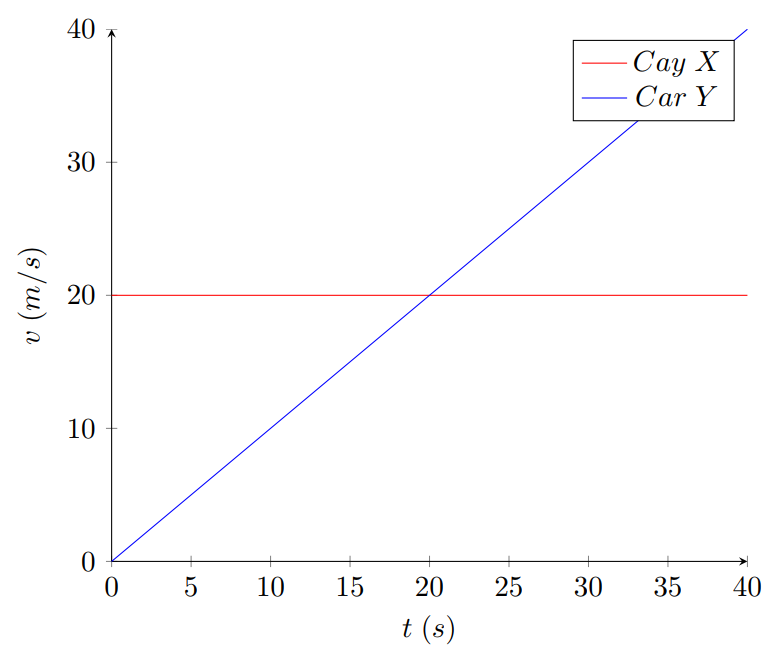
\includegraphics{Figures/Figure11}
\\
At time t=0, car X traveling with speed $v_0$ passes car Y, which is just starting to move. Both cars then travel on two parallel lanes of the same straight road. The graphs of speed $v$ versus time $t$ for both cars are shown above. Use this information for the next two questions.

%%%%%%%%%%%%%%%%%%%%%%%%%%%%%%%%%%
%%%%%%%%%%%%%%%%%%%%%%%%%%%%%%%%%%
%%%%%%%%%%%%%%%%%%%%%%%%%%%%%%%%%%

\begin{question}
(AP) Which of the following is true at time t=20 seconds?
\begin{enumerate}[label=(\alph*)]
    \item Car Y is behind car X
    \item Car Y is passing car X
    \item Car Y is in front of Car X
    \item Both Cars have the same acceleration
    \item Car X is accelerating faster than car Y
\end{enumerate}
\end{question}

\begin{solution}
A (hint: the area underneath v(t) is position)
\end{solution}

%%%%%%%%%%%%%%%%%%%%%%%%%%%%%%%%%%
%%%%%%%%%%%%%%%%%%%%%%%%%%%%%%%%%%
%%%%%%%%%%%%%%%%%%%%%%%%%%%%%%%%%%
\newpage
\begin{question}
(AP) From time $t=0$ to time $t=40\;seconds$, the areas under both curves are equal. Therefore, which of the following is true at time $t=40\;seconds$?
\begin{enumerate}[label=(\alph*)]
    \item Car Y is behind car X
    \item Car Y is passing car X
    \item Car Y is in front of Car X
    \item Both Cars have the same acceleration
    \item Car X is accelerating faster than car Y
\end{enumerate}
\end{question}

\begin{solution}
B (hint: equal areas mean currently, they're in the same position)
\end{solution}

%%%%%%%%%%%%%%%%%%%%%%%%%%%%%%%%%%
%%%%%%%%%%%%%%%%%%%%%%%%%%%%%%%%%%
%%%%%%%%%%%%%%%%%%%%%%%%%%%%%%%%%%

\begin{question}
(AP) A body moving in the positive x direction passes the origin at time $t=0$. Between $t=0$ and $t=1\;sec$, the body has a constant speed of $24\frac{m}{s}$. At $t=1\;sec$ the body is given a constant acceleration of 6 meters per second squared in the negative x direction. The positive x of the body at t=11 seconds is:
\begin{multicols}{5}
\begin{enumerate}[label=(\alph*)]
    \item +99 m
    \item +36 m
    \item -36 m
    \item -75 m
    \item -99 m
\end{enumerate}
\end{multicols}
\end{question}

\begin{solution}
C (Hint: use (1.3))
\end{solution}

%%%%%%%%%%%%%%%%%%%%%%%%%%%%%%%%%%
%%%%%%%%%%%%%%%%%%%%%%%%%%%%%%%%%%
%%%%%%%%%%%%%%%%%%%%%%%%%%%%%%%%%%

\begin{question}
(AP) An object released from rest at time t=0 slides down a frictionless incline a distance of 1 meter during the first second. The distance traveled by the object during the time itnerval from t=1 second to t=2 seconds is:
\begin{multicols}{5}
\begin{enumerate}[label=(\alph*)]
    \item 1 m
    \item 2 m
    \item 3 m
    \item 4 m
    \item 5 m
\end{enumerate}
\end{multicols}
\end{question}

\begin{solution}
C (Hint: The acceleration due to gravity isn't g!)
\end{solution}

%%%%%%%%%%%%%%%%%%%%%%%%%%%%%%%%%%
%%%%%%%%%%%%%%%%%%%%%%%%%%%%%%%%%%
%%%%%%%%%%%%%%%%%%%%%%%%%%%%%%%%%%

\begin{question}
(AP) Two people are in a boat that is capable of a maximum speed of 5 kilometers per hour in still water, and wish to cross a river 1 kilometer wide to a point directly across from their starting point. If the speed of the water in the river is 5 kilometers per hour, how much time is required for the crossing?
\begin{multicols}{5}
\begin{enumerate}[label=(\alph*)]
    \item 0.05 hr
    \item 0.1 hr
    \item 1 hr
    \item 10 hr
    \item \small{impossible}
\end{enumerate}
\end{multicols}
\end{question}

\begin{solution}
E (Hint: This is actually a stupid question. Use common sense!)
\end{solution}

%%%%%%%%%%%%%%%%%%%%%%%%%%%%%%%%%%
%%%%%%%%%%%%%%%%%%%%%%%%%%%%%%%%%%
%%%%%%%%%%%%%%%%%%%%%%%%%%%%%%%%%%

\begin{question}
(AP) A projectile is fired from the surface of the Earth with a speed of 200 meters per second at an angle of $30\deg$ above the horizontal. If the ground is level, what is the maximum height reached by the projectile?
\begin{multicols}{5}
\begin{enumerate}[label=(\alph*)]
    \item 5 m
    \item 10 m
    \item 500 m
    \item 1000 m
    \item 2000 m
\end{enumerate}
\end{multicols}
\end{question}

\begin{solution}
C (Hint: Velocity at the top of the trajectory is zero!)
\end{solution}

%%%%%%%%%%%%%%%%%%%%%%%%%%%%%%%%%%
%%%%%%%%%%%%%%%%%%%%%%%%%%%%%%%%%%
%%%%%%%%%%%%%%%%%%%%%%%%%%%%%%%%%%

\begin{question}
(AP) A rock is dropped from the top of a 45 meter tower, and at the same time a ball is thrown from the top of the tower in a horizontal direction. Air resistance is negligible. The ball and the rock hit the ground a distance of 30 meters apart. The horizontal velocity of the ball thrown was most nearly:
\begin{multicols}{5}
\begin{enumerate}[label=(\alph*)]
    \item 5 m/s
    \item 11 m/s
    \item 14.1 m/s
    \item 20 m/s
    \item 28.3 m/s
\end{enumerate}
\end{multicols}
\end{question}

\begin{solution}
B (Hint: First, you'll need to figure out the time it took, then solve for the speed)
\end{solution}

%%%%%%%%%%%%%%%%%%%%%%%%%%%%%%%%%%
%%%%%%%%%%%%%%%%%%%%%%%%%%%%%%%%%%
%%%%%%%%%%%%%%%%%%%%%%%%%%%%%%%%%%

\begin{question}
(AP) In the absense of air friction, an object dropped near the surface of the Earth experiences a constant acceleration of about $9.8\frac{m}{s^2}$. This means that the
\begin{enumerate}[label=(\alph*)]
    \item speed of the object increases 9.8 m/s during each second
    \item speed of the object as it falls is 9.8 m/s
    \item object falls 9.8 meters during each second
    \item object falls 9.8 meters during the first second only
\end{enumerate}

\end{question}

\begin{solution}
A (Hint: Go over what acceleration is again)
\end{solution}


%%%%%%%%%%%%%%%%%%%%%%%%%%%%%%%%%%
%%%%%%%%%%%%%%%%%%%%%%%%%%%%%%%%%%
%%%%%%%%%%%%%%%%%%%%%%%%%%%%%%%%%%

\begin{question}
(AP) A 500 kilogram sports car accelerates uniformly from rest, reaching a speed of 30 meters per second in 6 seconds. During the 6 seconds, the car has traveled a distance of:
\begin{multicols}{5}
\begin{enumerate}[label=(\alph*)]
    \item 15 m
    \item 30 m
    \item 60 m
    \item 90 m
    \item 180 m
\end{enumerate}
\end{multicols}
\end{question}

\begin{solution}
D (Hint: First solve for acceleration, then solve for distance)
\end{solution}


%%%%%%%%%%%%%%%%%%%%%%%%%%%%%%%%%%
%%%%%%%%%%%%%%%%%%%%%%%%%%%%%%%%%%
%%%%%%%%%%%%%%%%%%%%%%%%%%%%%%%%%%

\begin{question}
(AP) An object is shot vertically upward into the air with a positive velocity. Which of the following correctly describes the velocity and acceleration of the object at its maximum elevation?

\begin{tabular}{ |c|c|c| } 
\hline
       & Velocity & Acceleration \\ 
 A     & Positive & Positive \\ 
 B     & Zero & Zero \\ 
 C     & Negative & Negative \\ 
 D     & Zero & Negative \\ 
 E     & Positive & Negative \\
\end{tabular}

\end{question}

\begin{solution}
E (Hint: It's going up, but slowing down!)
\end{solution}

%%%%%%%%%%%%%%%%%%%%%%%%%%%%%%%%%%
%%%%%%%%%%%%%%%%%%%%%%%%%%%%%%%%%%
%%%%%%%%%%%%%%%%%%%%%%%%%%%%%%%%%%
\newpage
\begin{question}
(AP) A spring-loaded gun can fire a projectile to a height h if it is fired straight up. If the same gun is pointed at an angle of $45\deg$ from the vertical, what maximum height can now be reached by the projectile?
\begin{multicols}{5}
\begin{enumerate}[label=(\alph*)]
    \item $\frac{h}{4}$
    \item $\frac{h}{2\sqrt{2}}$
    \item $\frac{h}{2}$
    \item $\frac{h}{\sqrt{2}}$
    \item $h$
\end{enumerate}
\end{multicols}
\end{question}

\begin{solution}
D (Hint: It's very similar to 1.3.8)
\end{solution}

%%%%%%%%%%%%%%%%%%%%%%%%%%%%%%%%%%
%%%%%%%%%%%%%%%%%%%%%%%%%%%%%%%%%%
%%%%%%%%%%%%%%%%%%%%%%%%%%%%%%%%%%

\begin{question}
(AP) The velocity of a projectile at launch has a horizontal component $v_h$ and a vertical component $v_v$. Air resistance is negligible. When the projectile is at the highest point of its trajectory, which of the following show the vertical and horizontal components of its velocity and the vertical component of its acceleration?

\begin{tabular}{ |c|c|c|c| } 
 \hline
       & Vertical Velocity & Horizontal Velocity & Vertical Acceleration \\ 
 A     & $v_v$ & $v_h$ & 0\\  
 B     & $v_v$ & 0 & 0\\ 
 C     & 0 & $v_h$ & 0\\ 
 D     & 0 & 0 & g\\ 
 E     & 0 & $v_h$ & g\\ 
 \hline
\end{tabular}

\end{question}

\begin{solution}
E (Hint: It's still moving forward, but it's not moving up anymore. Something's pulling it down!)
\end{solution}

%%%%%%%%%%%%%%%%%%%%%%%%%%%%%%%%%%
%%%%%%%%%%%%%%%%%%%%%%%%%%%%%%%%%%
%%%%%%%%%%%%%%%%%%%%%%%%%%%%%%%%%%

\begin{question}
(AP) A target $T$ lies flat on the ground 3 m from the side of a building that  is 10 m tall. A student rolls a ball off the horizontal roof of the building in the direction of the target. Air Resistance is negligible. The horizontal speed with which the ball must leave the roof if it is to strike the target is most nearly:

\begin{multicols}{5}
\begin{enumerate}[label=(\alph*)]
    \item $\frac{3}{10}\frac{m}{s}$
    \item $\sqrt{2}\frac{m}{s}$
    \item $\frac{3}{\sqrt{2}}\frac{m}{s}$
    \item $3\frac{m}{s}$
    \item $10\sqrt{\frac{10}{3}}\frac{m}{s}$
\end{enumerate}
\end{multicols}

\end{question}

\begin{solution}
C (Hint: Solve for time, then solve for velocity)
\end{solution}

%%%%%%%%%%%%%%%%%%%%%%%%%%%%%%%%%%
%%%%%%%%%%%%%%%%%%%%%%%%%%%%%%%%%%
%%%%%%%%%%%%%%%%%%%%%%%%%%%%%%%%%%

\begin{question}
(AP) An object is dropped from rest from the top of a 400 m cliff on Earth. If air resistance is negligible, what is the distance the object travels during the first 6 s of its fall?

\begin{multicols}{5}
\begin{enumerate}[label=(\alph*)]
    \item 30 m
    \item 60 m
    \item 120 m
    \item 180 m
    \item 360 m
\end{enumerate}
\end{multicols}

\end{question}

\begin{solution}
D (Hint: For problems like this, double check by making sure the time it takes to fall 300 metres is over 6 seconds)
\end{solution}

%%%%%%%%%%%%%%%%%%%%%%%%%%%%%%%%%%
%%%%%%%%%%%%%%%%%%%%%%%%%%%%%%%%%%
%%%%%%%%%%%%%%%%%%%%%%%%%%%%%%%%%%
\newpage
\begin{question}
(AP) A student is testing the kinematic equations for uniformly accelerated motion by measuring the time it takes for light-weight plastic balls to fall to the floor from a height of 3 m in the lab. The student predicts the time to fall using g as 9.80 m/s2 but finds the measured time to be 35\% greater. Which of the following is the most likely cause of the large percent error?   

\begin{enumerate}[label=(\alph*)]
    \item The acceleration due to gravity is 70\% greater than $9.8\frac{m}{s^2}$
    \item The acceleration due to gravity is 70\% less than $9.8\frac{m}{s^2}$
    \item Air resistance increases the downward acceleration
    \item The acceleration of the plastic balls is not uniform
    \item The plastic balls are not truly spherical
\end{enumerate}

\end{question}

\begin{solution}
D (Hint: Use a process of elimination!)
\end{solution}

%%%%%%%%%%%%%%%%%%%%%%%%%%%%%%%%%%
%%%%%%%%%%%%%%%%%%%%%%%%%%%%%%%%%%
%%%%%%%%%%%%%%%%%%%%%%%%%%%%%%%%%%

\begin{question}
(AP) An object is thrown with velocity v from the edge of a cliff above level ground. Neglect air resistance. In order for the object to travel a maximum horizontal distance from the cliff before hitting the ground, the throw should be at an angle $\theta$ with respect to the horizontal of

\begin{enumerate}[label=(\alph*)]
    \item Greater than $60\deg$ above the horizontal
    \item greater than $45\deg$ but less than $60\deg$ above the horizontal
    \item greater than zero but less than $45\deg$ above the horizontal
    \item zero
    \item greater than zero but less than $45\deg$ below the horizontal
\end{enumerate}

\end{question}

\begin{solution}
C (Hint: If two trajectories ever cross paths, the one with the higher x velocity will land furthest)
\end{solution}

%%%%%%%%%%%%%%%%%%%%%%%%%%%%%%%%%%
%%%%%%%%%%%%%%%%%%%%%%%%%%%%%%%%%%
%%%%%%%%%%%%%%%%%%%%%%%%%%%%%%%%%%
\newpage
Starting from rest, a vehicle accelerates on a straight level road at the rate of $4 \frac{m}{s^2}$ for 5 seconds. Use this information for the next two questions:

%%%%%%%%%%%%%%%%%%%%%%%%%%%%%%%%%%
%%%%%%%%%%%%%%%%%%%%%%%%%%%%%%%%%%
%%%%%%%%%%%%%%%%%%%%%%%%%%%%%%%%%%

\begin{question}
(AP) What is the speed of the vehicle at the end of this time interval?

\begin{multicols}{5}
\begin{enumerate}[label=(\alph*)]
    \item 1.3 m/s
    \item 10 m/s
    \item 20 m/s
    \item 80 m/s
    \item 100 m/s
\end{enumerate}
\end{multicols}
\end{question}

\begin{solution}
C (Hint: Use 1.2)
\end{solution}

%%%%%%%%%%%%%%%%%%%%%%%%%%%%%%%%%%
%%%%%%%%%%%%%%%%%%%%%%%%%%%%%%%%%%
%%%%%%%%%%%%%%%%%%%%%%%%%%%%%%%%%%

\begin{question}
(AP) What is the total distance the vehicle travels during this time interval?
\begin{multicols}{5}
\begin{enumerate}[label=(\alph*)]
    \item 10 m
    \item 20 m
    \item 25 m
    \item 40 m
    \item 50 m
\end{enumerate}
\end{multicols}
\end{question}

\begin{solution}
E (Hint: Use 1.3)
\end{solution}

%%%%%%%%%%%%%%%%%%%%%%%%%%%%%%%%%%
%%%%%%%%%%%%%%%%%%%%%%%%%%%%%%%%%%
%%%%%%%%%%%%%%%%%%%%%%%%%%%%%%%%%%

\begin{question}
(AP) If air resistance is negligible, the speed of a 2 kg sphere that falls from rest through a vertical displacement of 0.2 m is most nearly
\begin{multicols}{5}
\begin{enumerate}[label=(\alph*)]
    \item 1 m/s
    \item 2 m/s
    \item 3 m/s
    \item 4 m/s
    \item 5 m/s
\end{enumerate}
\end{multicols}
\end{question}

\begin{solution}
E (Hint: Use 1.3)
\end{solution}

%%%%%%%%%%%%%%%%%%%%%%%%%%%%%%%%%%
%%%%%%%%%%%%%%%%%%%%%%%%%%%%%%%%%%
%%%%%%%%%%%%%%%%%%%%%%%%%%%%%%%%%%

\begin{question}
(AP) A projectile is launched from level ground with an initial speed $v_0$ at an angle $\theta$ with the horizontal. If air resistance is negligible, how long will the projectile remain in the air?
\begin{multicols}{5}
\begin{enumerate}[label=(\alph*)]
    \item $\frac{2v_0}{g}$
    \item $\frac{2v_0cos(\theta)}{g}$
    \item $\frac{v_0cos(\theta)}{g}$
    \item $\frac{v_0sin(\theta)}{g}$
    \item $\frac{2v_0sin(\theta)}{g}$
\end{enumerate}
\end{multicols}
\end{question}

\begin{solution}
E (Hint: The original and final speed is the same, due to the symmetry of the parabola)
\end{solution}

%%%%%%%%%%%%%%%%%%%%%%%%%%%%%%%%%%
%%%%%%%%%%%%%%%%%%%%%%%%%%%%%%%%%%
%%%%%%%%%%%%%%%%%%%%%%%%%%%%%%%%%%

\begin{question}
(AP) An object of unknown mass is initially at rest and dropped from a height h. It reaches the ground with a velocity $v_1$ The same object is then raised again to the same height h but this time is thrown downward with velocity $v_1$ It now reaches the ground with a new velocity $v_2$. How is $v_2$ related to $v_1$? 
\begin{multicols}{5}
\begin{enumerate}[label=(\alph*)]
    \item $v_2 = \frac{v_1}{2}$
    \item $v_2 = v_1$
    \item $v_2 = \frac{v_1}{\sqrt{2}}$
    \item $v_2 = 2v_1$
    \item $v_2 = 4v_1$
\end{enumerate}
\end{multicols}
\end{question}

\begin{solution}
E (Hint: Use 1.4 to solve solve for $v_1$ then use 1.4 again to solve for $v_2$ in terms of $v_1$. Then substitute.)
\end{solution}

%%%%%%%%%%%%%%%%%%%%%%%%%%%%%%%%%%
%%%%%%%%%%%%%%%%%%%%%%%%%%%%%%%%%%
%%%%%%%%%%%%%%%%%%%%%%%%%%%%%%%%%%
\newpage
\begin{question}
The velocity function for an object falling from rest under the influence of gravity and air resistance is shown below. Which of the following statements about x(t) are consistent with this velocity function?

% \begin{tikzpicture}

% \begin{axis}[
%     axis lines = left,
%     xlabel = $t\;(s)$,
%     ylabel = {$v\;(m/s)$},
% ]

% %Below the black is defined
% \addplot [
%     domain=5:100,
%     samples=100, 
%     color=black,
% ]
% {0.3};
% \addlegendentry{terminal velocity}
% %Below the red is defined
% \addplot [
%     domain=0:100,
%     range=0:2,
%     samples=100, 
%     color=red,
% ]
% {x/(10+3.333*x)};

% %Below the black is defined
% \addplot [
%     domain=1:100,
%     samples=100, 
%     color=white,
% ]
% {0.5};

% \end{axis}
% \end{tikzpicture}
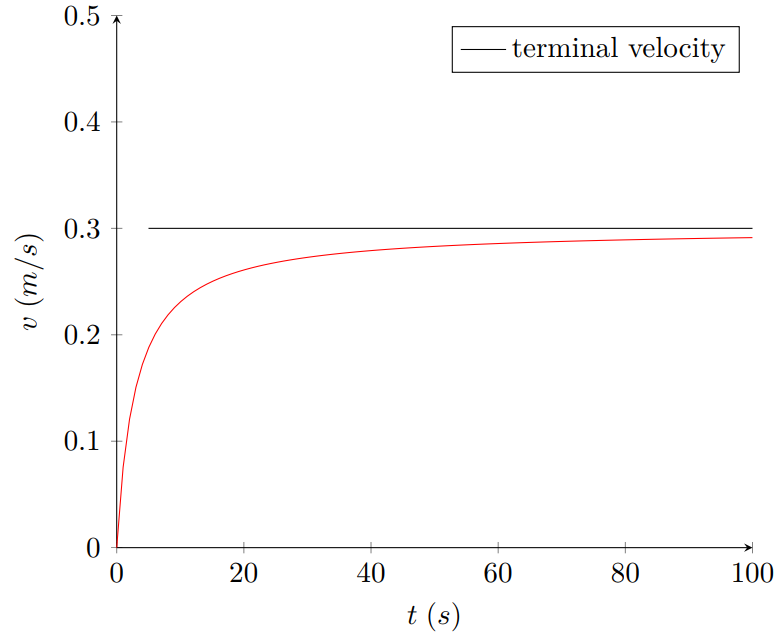
\includegraphics{Figures/Figure12}

\begin{tabular}{ |c|c|c|c| } 
 \hline
       & Y-Intercept & Starting Acceleration & Asymptote \\ 
 A     & Zero & Positive & Slant (Oblique)\\  
 B     & Positive & Positive & Horizontal\\ 
 C     & Zero & Negative & Slant (Oblique)\\ 
 D     & Negative & Negative & Horizontal\\ 
 E     & Zero & Positive & No\\ 
 \hline
\end{tabular}

\end{question}

\begin{solution}
A (Hint: Sketch it out!)
\end{solution}

%%%%%%%%%%%%%%%%%%%%%%%%%%%%%%%%%%
%%%%%%%%%%%%%%%%%%%%%%%%%%%%%%%%%%
%%%%%%%%%%%%%%%%%%%%%%%%%%%%%%%%%%

\begin{question}
A particle moves along the x-axis with a nonconstant acceleration described by $a=12t$, where a is in meters per second squared and t is in seconds. If the particle starts from rest so that its speed $v$ and position $x$ are zero when t=0, where is it located when $t=2\;sec$?
\begin{multicols}{5}
\begin{enumerate}
    \item 5 m
    \item 10 m
    \item 500 m
    \item 1000 m
    \item 2000 m
\end{enumerate}
\end{multicols}
\end{question}

\begin{solution}
B (Hint: take the integral two times!)
\end{solution}

%%%%%%%%%%%%%%%%%%%%%%%%%%%%%%%%%%
%%%%%%%%%%%%%%%%%%%%%%%%%%%%%%%%%%
%%%%%%%%%%%%%%%%%%%%%%%%%%%%%%%%%%
\newpage
\begin{question}
Vectors $v_1$ and $v_2$ shown below have equal magnitudes. The vectors represent the velocities of an object at times $t_1$, and $t_2$, respectively. The average acceleration of the object between time $t_1$ and $t_2$ was directed:

% \begin{tikzpicture}
%   \draw[thin,gray!40] (-2,-2) grid (2,2);
%   \draw[<->] (-2,0)--(2,0) node[right]{$E$};
%   \draw[<->] (0,-2)--(0,2) node[above]{$N$};
%   \draw[line width=2pt,blue,-stealth](0,0)--(1,0.5) node[anchor=south west]{$\boldsymbol{v_1}$};
%   \draw[line width=2pt,red,-stealth](0,0)--(0,1) node[anchor=north east]{$\boldsymbol{v_2}$};
% \end{tikzpicture}
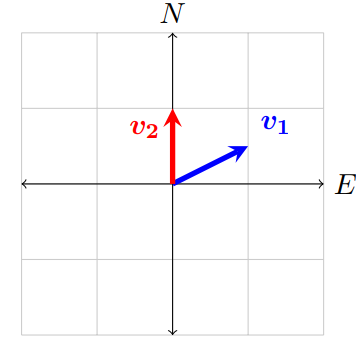
\includegraphics{Figures/Figure13}
\begin{multicols}{4}
\begin{enumerate}[label=(\alph*)]
    \item North
    \item West
    \item North of East
    \item North of West
\end{enumerate}
\end{multicols}

\end{question}

\begin{solution}
D (Hint: We're not looking at the location of $v$. We're looking at how $v$ changes.
\end{solution}

%%%%%%%%%%%%%%%%%%%%%%%%%%%%%%%%%%
%%%%%%%%%%%%%%%%%%%%%%%%%%%%%%%%%%
%%%%%%%%%%%%%%%%%%%%%%%%%%%%%%%%%%

\begin{question}
An object is thrown vertically upward in a region where g is constant and air resistance is negligible. Its speed is recorded from the moment it leaves the thrower's hand until it reaches its maximum height. Which of the following graphs best represent the object's speed $v$ versus time $t$ \footnote{If you can't distinguish between the colors, A, B, C, D are labelled in order of the end behaviour of each line}

% \begin{tikzpicture}
% \begin{axis}[
%     axis lines = left,
%     xlabel = $t$,
%     ylabel = {$v$},
% ]

% %A
% \addplot [
%     domain=0:1,
%     samples=100, 
%     color=blue,
% ]
% {e^x-1};
% \addlegendentry{A}

% %B
% \addplot [
%     domain=0:1,
%     samples=100, 
%     color=red,
% ]
% {x};
% \addlegendentry{B}

% %C
% \addplot [
%     domain=0:1,
%     samples=100, 
%     color=black,
% ]
% {ln(x+1)};
% \addlegendentry{C}

% %D
% \addplot [
%     domain=0:1,
%     samples=100, 
%     color=green,
% ]
% {1-x};
% \addlegendentry{D}

% \end{axis}
% \end{tikzpicture}

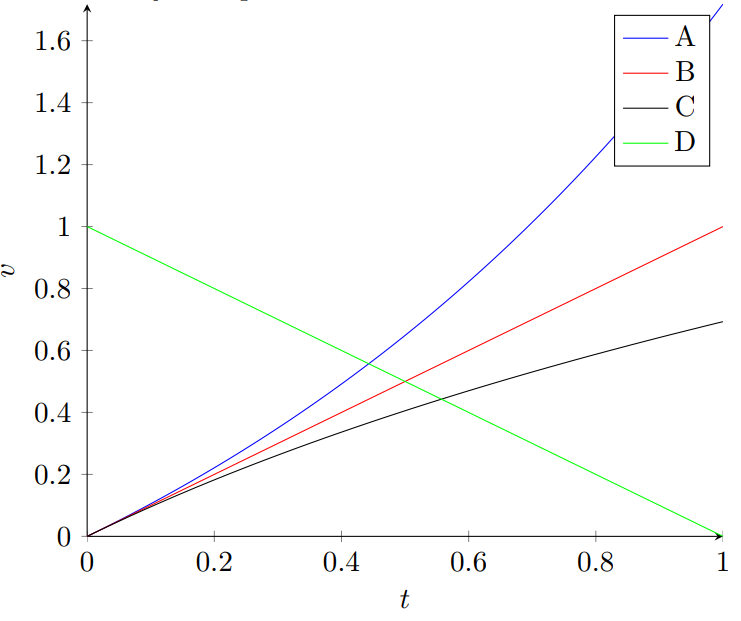
\includegraphics{Figures/Figure14}

\end{question}
\newpage
An object moving in a straight line has a velocity v in meters per second that varies with time t in seconds according to the following function: $v=4+0.5t^2$. Use this information to answer the next two questions:

%%%%%%%%%%%%%%%%%%%%%%%%%%%%%%%%%%
%%%%%%%%%%%%%%%%%%%%%%%%%%%%%%%%%%
%%%%%%%%%%%%%%%%%%%%%%%%%%%%%%%%%%

\begin{question}
The instantaneous acceleration of the object at t = 2 seconds is:
\begin{multicols}{5}
\begin{enumerate}
    \item $2\frac{m}{s^2}$
    \item $4\frac{m}{s^2}$
    \item $5\frac{m}{s^2}$
    \item $6\frac{m}{s^2}$
    \item $8\frac{m}{s^2}$
\end{enumerate}
\end{multicols}
\end{question}

\begin{solution}
A (Acceleration is the first derivative of velocity)
\end{solution}

%%%%%%%%%%%%%%%%%%%%%%%%%%%%%%%%%%
%%%%%%%%%%%%%%%%%%%%%%%%%%%%%%%%%%
%%%%%%%%%%%%%%%%%%%%%%%%%%%%%%%%%%

\begin{question}
The displacement of the object between t=0 and t=6 seconds is:
\begin{multicols}{5}
\begin{enumerate}
    \item 22 m
    \item 28 m
    \item 40 m
    \item 42 m
    \item 60 m
\end{enumerate}
\end{multicols}
\end{question}

\begin{solution}
E (Take the definite integral with 0 and 6 as bounds!)
\end{solution}

%%%%%%%%%%%%%%%%%%%%%%%%%%%%%%%%%%
%%%%%%%%%%%%%%%%%%%%%%%%%%%%%%%%%%
%%%%%%%%%%%%%%%%%%%%%%%%%%%%%%%%%%

\begin{question}
The position of an object is given by the equation $x=3t^2+1.5t+4.5$ where x is in meters and t is in seconds. What is the instantaneous acceleration of the object at $t=3\;sec$?

\begin{multicols}{5}
\begin{enumerate}
    \item $3 \frac{m}{s^2}$
    \item $6 \frac{m}{s^2}$
    \item $9 \frac{m}{s^2}$
    \item $19.5 \frac{m}{s^2}$
    \item $36 \frac{m}{s^2}$
\end{enumerate}
\end{multicols}
\end{question}

\begin{solution}
B (Hint: Acceleration is the second derivative of position)
\end{solution}

%%%%%%%%%%%%%%%%%%%%%%%%%%%%%%%%%%
%%%%%%%%%%%%%%%%%%%%%%%%%%%%%%%%%%
%%%%%%%%%%%%%%%%%%%%%%%%%%%%%%%%%%

\begin{question}
At a particular instant, a stationary observer on the ground sees a package falling with a speed of $v_1$ at an angle to the vertical. To a pilot flying horizontaly at constant speed relative to the ground, the package appears to be falling vertically with a speed $v_2$ at that instant. What is the speed of the pilot relative to the ground?

\begin{multicols}{5}
\begin{enumerate}
    \item $v_1+v_2$
    \item $v_1-v_2$
    \item $v_2-v_1$
    \item $\sqrt{v_1^2-v_2^2}$
    \item $\sqrt{v_1^2+v_2^2}$
\end{enumerate}
\end{multicols}
\end{question}

\begin{solution}
D (Hint: Pythagorean Theorem!)
\end{solution}

%%%%%%%%%%%%%%%%%%%%%%%%%%%%%%%%%%
%%%%%%%%%%%%%%%%%%%%%%%%%%%%%%%%%%
%%%%%%%%%%%%%%%%%%%%%%%%%%%%%%%%%%
%%%%%%%%%%%%%%%%%%%%%%%%%%%%%%%%%%
%%%%%%%%%%%%%%%%%%%%%%%%%%%%%%%%%%
%%%%%%%%%%%%%%%%%%%%%%%%%%%%%%%%%%
%%%%%%%%%%%%%%%%%%%%%%%%%%%%%%%%%%
%%%%%%%%%%%%%%%%%%%%%%%%%%%%%%%%%%
%%%%%%%%%%%%%%%%%%%%%%%%%%%%%%%%%%
%%%%%%%%%%%%%%%%%%%%%%%%%%%%%%%%%%
%%%%%%%%%%%%%%%%%%%%%%%%%%%%%%%%%%
%%%%%%%%%%%%%%%%%%%%%%%%%%%%%%%%%%
%%%%%%%%%%%%%%%%%%%%%%%%%%%%%%%%%%
%%%%%%%%%%%%%%%%%%%%%%%%%%%%%%%%%%
%%%%%%%%%%%%%%%%%%%%%%%%%%%%%%%%%%